% !TEX TS-program = xelatex
% !TEX encoding = UTF-8 Unicode
% !Mode:: "TeX:UTF-8"
\documentclass{resume}
%\documentclass[8pt]{article}
%\usepackage{zh_CN-Adobefonts_external} % Simplified Chinese Support using external fonts (./fonts/zh_CN-Adobe/)
\usepackage{zh_CN-Adobefonts_internal} % Simplified Chinese Support using system fonts
\usepackage{linespacing_fix} % disable extra space before next section
\usepackage{cite}
\usepackage[colorlinks,linkcolor=blue,anchorcolor=blue,citecolor=green,urlcolor=blue]{hyperref}
\usepackage{amssymb}
\usepackage{amsmath}
\usepackage{color}
% \definecolor{usercolor}{rgb}{0.5,0.8.0.7}
%for header image
\usepackage{graphicx}
\usepackage{tikz} %用于定位照片
\usetikzlibrary{calc}
%for floating figures
\usepackage{wrapfig}
\usepackage{float}
%\floatstyle{boxed}
%\restylefloat{figure}
\usepackage{geometry}
\geometry{left=1.5cm,right=1.5cm,top=1cm,bottom=0.1cm}

% \newcommand{\vcenteredinclude}[1]{\begingroup
% \setbox0=\hbox{\hspace*{-0.1cm}\includegraphics[width=0.1cm]{#1}}%
% \parbox{\wd0}{\box0}\endgroup}


\begin{document}
\pagenumbering{gobble} % suppress displaying page number

\name{ 张\hspace{0.1cm}贵\hspace{0.1cm}瑞 }

% {E-mail}{mobilephone}{homepage}
% be careful of _ in emaill address
{\centerline{\contactInfo{17781444956@163.com}{177-8144-4956}{1997-02-23}}}
{\qquad \qquad \qquad \qquad 
{GitHub:\href{https://github.com/freesix}{https://github.com/freesix}}\quad
个人博客:\href{https://freesix.github.io/}{freesix.github.io}}

\begin{tikzpicture}[remember picture,overlay]
  \node[anchor = north east] at ($(current page.north east)+(-2cm,-1.2cm)$){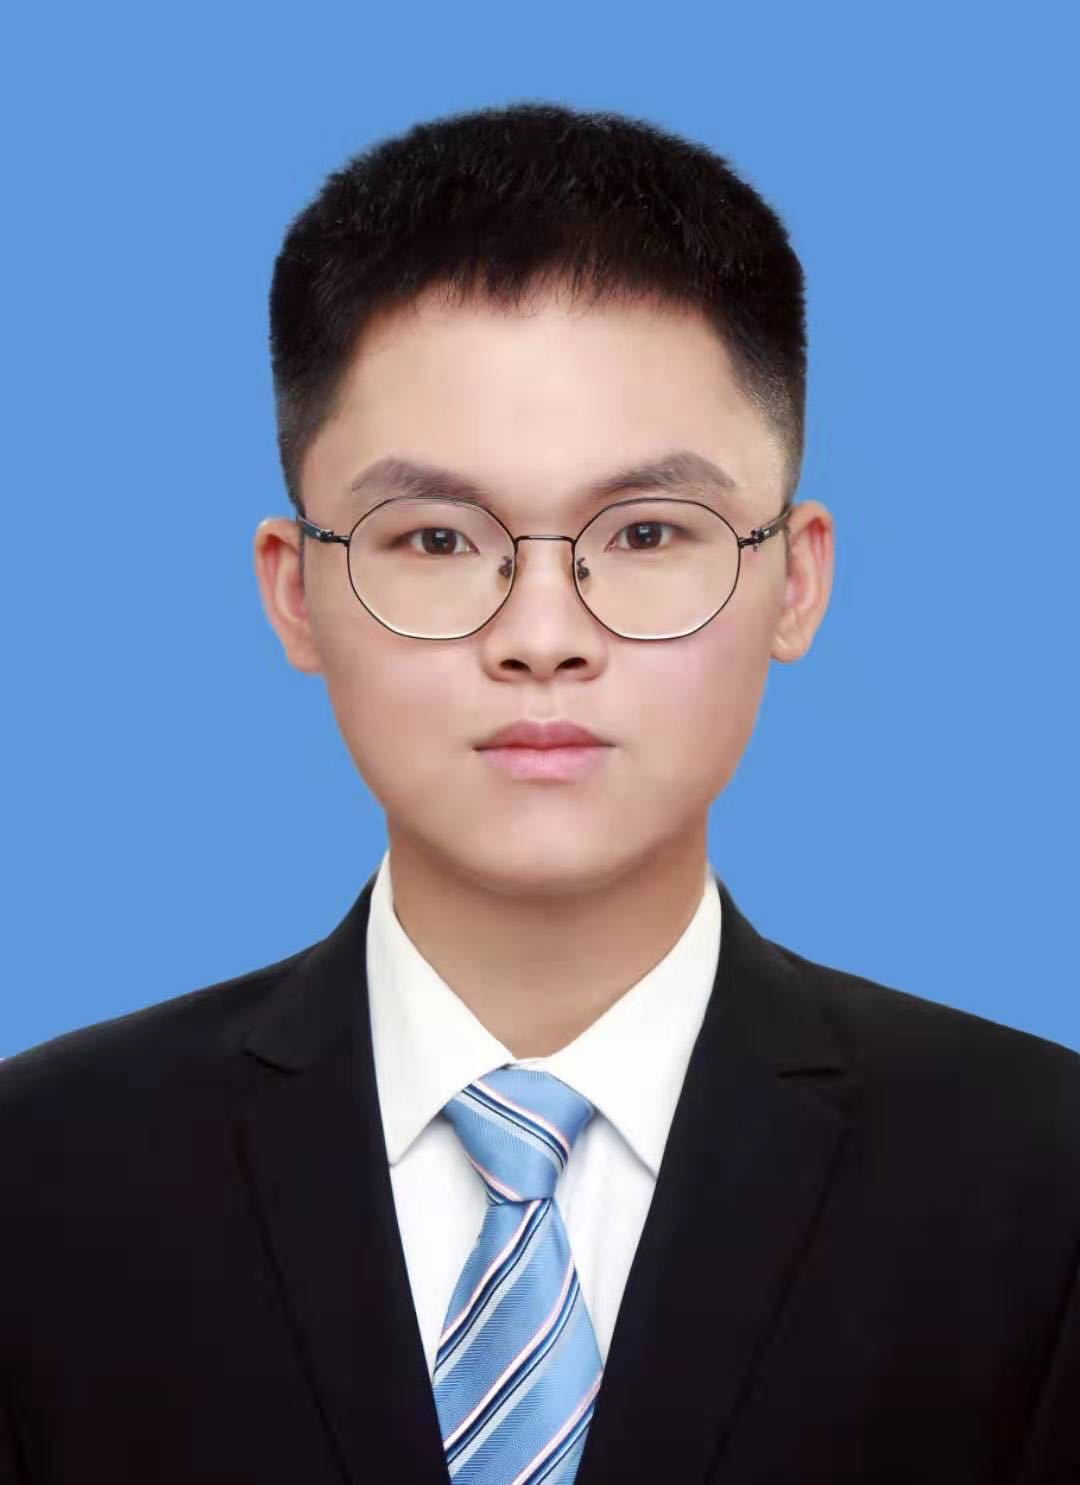
\includegraphics[width=2.5cm]{images/照片.jpg}};
\end{tikzpicture}
% \centerline{\includegraphics[width=0.2cm]{imazhen.jpg}}

% {E-mail}{mobilephone}
% keep the last empty braces!
%\contactInfo{xxx@yuanbin.me}{(+86) 131-221-87xxx}{}
求职意向:\textbf{SLAM算法工程师、3D算法工程师等}


\section{\textcolor[RGB]{50,50,190}{\faGraduationCap 教育背景}}

\datedsubsection{\textbf{西南民族大学}, 电气工程学院}{2021年9月 -- 2024年6月}
\textit{硕士}\ \ 电子信息专业 \qquad \qquad
\textcolor[RGB]{80,100,190}{\textbf{研究方向}}:
SLAM、图像拼接、点云配准


\datedsubsection{\textbf{上海工程技术大学}, 电气工程学院}{2016年9月 -- 2020年7月}
\textit{学士}\ \ 自动化专业

\section{\textcolor[RGB]{50,50,190}{\faBriefcase 工作经历}}

\datedsubsection{\textbf{上海芯圣电子股份有限公司}}{2020年5月 -- 2021年8月}
FAE工程师(正式工作)\qquad 总经理室
\begin{itemize}
  \item 负责公司产品的技术支持,包括技术咨询、技术培训、技术支持等。
  % \item 发挥FAE的技术能力和经验,协助客户工程人员在方案中导入芯片。
  % \item 嵌入式软件开发,如血氧仪、触摸控制板、锂电充手电等消费类电子产品开发。
  \item 便携式血氧仪和公司触摸控制板的算法优化和改进,如滤波算法、异常处理等。
    % \item 负责客户技术人员的技术培训,帮助其提高对产品的认知,培养对我方产品的使用习惯。
  % \item 收集客户需求和产品反馈,协助产品部门和推动产品的改进。
  \item 负责华东片区大客户,如鱼跃医疗、科大讯飞、小米等公司的现场技术支持。
  % \item 内部营销人员、新员工的技术培训,围绕本公司产品撰写对外教材和录制培训视频。
  \item 产品的应用开发,编写芯片例程、设计demo板。
\end{itemize}

\section{\textcolor[RGB]{50,50,190}{\faAlignLeft 实习经历}}

\datedsubsection{\textbf{第六镜科技(成都)有限公司}}{2023年11月 -- 至今}
3D算法工程师\qquad \qquad \quad AI技术部
\begin{itemize}
  \item 负责铁轨轮廓结构光3D重建项目的光条中心线提取、点云处理部分算法。
  \item 改进steger算法,适应高速采集工况下的应用。
\end{itemize}

\section{\textcolor[RGB]{50,50,190}{\faCogs\ 技能}}
% increase linespacing [parsep=0.5ex]
\begin{itemize}[parsep=0.5ex]
  \item Python、C、C++、LaTex、Matlab、Linux、ROS2、Pytorch
  \item 了解李群李代数、对极几何、图优化、EKF、ESEKF等,对Eigen、g2o、OpenCV等有一定使用
  \item 了解LIO-SAM、Point-LIO、Far-planner、ORB\_SLAM3框架
  \item 对GNN和图匹配相关算法有一定了解,并用于点云配准的研究,学习过Point-GNN等框架
  % \item 

\end{itemize}


\section{\textcolor[RGB]{50,50,190}{\faUsers\ 科研 / 项目经历}}

% \end{itemize}

\datedsubsection{\textbf{多视角图像拼接补全算法设计}--西南民族大学(横向项目)}{2022年12月 -- 至今}
\textcolor[RGB]{80,100,190}{\textbf{项目链接}}:\hyperlink{https://github.com/freesix/GNN-martch}
{https://github.com/freesix/GNN-martch}

% \begin{itemize}
\textcolor[RGB]{80,100,190}{\textbf{项目简介}}:
将曲面上的16块CMOS芯片所成图像拼接成一幅完整且清晰的图像。解决成像平面和曲面之间的高度差
所带来的图像失焦、畸变、像素盲区等问题,\textbf{图像配准先进算法的研究和实现}。

\textcolor[RGB]{80,100,190}{\textbf{工作内容}}:
设计先进\textbf{图匹配算法}用于\textbf{图像拼接的配准步骤和点云配准},借助GNN、最大团匹配、
因子图分解等方法提升配准的精度和鲁棒性,提高对图像特征点离群值的筛选。
% 根据横向项目的需求制定技术路线,撰写需求分析、技术目标等文档,整体拼接算法路线制定,图像匹配
% 部分算法的研究和实现、深度模型的设计和训练等。后续估计失焦图像的PSF用于模糊图像恢复,对畸变
% 图像设计畸变模型估计畸变参数。

\textcolor[RGB]{80,100,190}{\textbf{工作成果}}:
论文$\ll$ Image Stitching with Weight Learnable Graph Matching Network$\gg$(暂定),
% 图像配准的性能远高于传统KNN+RANSAC算法或SuperGlue等学习方法。
提出了一种权重可学习的图注意力机制用于图像拼接的配准步骤,图像配准的性能优于传统的KNN+RANSAC
算法或SuperGlue等学习方法。

\datedsubsection{\textbf{便携式血氧仪算法和硬件改进}--上海芯圣电子股份有限公司}{2020年7月 -- 2021年8月}
% \begin{itemize}
\textcolor[RGB]{80,100,190}{\textbf{项目简介}}:
替换原有主控芯片为公司自研芯片,替换TS9514为传统电路来控制红光和红外探头,修改血氧信号处理算法,针对
异常工况修改代码、重新设计PCB以降低硬件成本。
% 提升血氧仪在不同测量状况下的测量准确率。对剧烈运动、手指放置不正确等异常增加修改相应程序。
% 主控芯片的改版,重新设计PCB以降低硬件成本。

\textcolor[RGB]{80,100,190}{\textbf{工作内容}}:
重构替换方案后的代码、硬件,改进优化算法,后续测试问题的跟进和解决等一系列工作。

\textcolor[RGB]{80,100,190}{\textbf{工作成果}}:
成功将自研芯片融入方案,改进算法和增加异常处理等,制作demo板并成功进入医疗器械审查阶段。

\datedsubsection{\textbf{锂电充手电开发}--上海芯圣电子股份有限公司}{2020年12月 -- 2021年8月}
% \begin{itemize}
\textcolor[RGB]{80,100,190}{\textbf{项目简介}}:
一款锂电充手电的项目立项开发。

\textcolor[RGB]{80,100,190}{\textbf{工作内容}}:
负责整体项目评估和框架搭建,完成项目的软件开发,与厂商硬件工程师合作共同完成项目开发。

\textcolor[RGB]{80,100,190}{\textbf{工作成果}}:
成功立项,完成AD、定时器、PWM等一系列模块代码设计。
% \\

\datedsubsection{\textbf{基于51单片机的声控光控感应灯}--上海工程技术大学(创新大赛)}{2017年10月 -- 2017年12月}

\textcolor[RGB]{80,100,190}{\textbf{项目简介}}:
校内电子设计大赛,根据题目要求设计一款可光控、声控且能够感应人体的感应灯。

\textcolor[RGB]{80,100,190}{\textbf{工作内容}}:
学习Altium Designer、Keil软件的使用,根据课题设计硬件电路和完成功能代码的编写。

\textcolor[RGB]{80,100,190}{\textbf{工作成果}}:
学会嵌入式有关软件的使用,顺利完成项目。
\section{\textcolor[RGB]{50,50,190}{\faPaperPlane\ 获奖和科研成果}}
% \begin{itemize}
研究生奖学金两次、本科生奖学金一次、本科校三等奖一次
% \end{itemize}
% \end{itemize\i\}
\section{\textcolor[RGB]{50,50,190}{\faChild\ 自我评价}}
拥有良好的自我驱动力,学习能力强,对激光slam、视觉slam、嵌入式软件开发、运动想象脑电、图像拼
接等领域均有不同程度的涉猎和研究。在实习、工作中表现出了组织和团队领导能力,一年多工作时间已成
为部门主要负责人。



%% Reference
%\newpage
%\bibliographystyle{IEEETran}
%\bibliography{mycite}
\end{document}
